\section{Аналитическая часть}

В данном разделе приводится краткий обзор предметной области. Описаны протоколы поддерживающие шифрование данных.


\subsection{Обзор предметной области}

\subsubsection{Модель OSI}

Модель OSI (Open Systems Interconnection) является концептуальным рамочным протоколом, разработанным Международной организацией по стандартизации (ISO), чтобы стандартизировать связь между различными компьютерными системами \cite{osi}. Она была определена в 1984 году и является основным принципом организации и реализации сетевых протоколов.

Модель OSI состоит из семи уровней, каждый из которых выполняет определенные функции для обеспечения надежной и эффективной коммуникации (см. рис \ref{fig:osi}).

\begin{figure}[h]
	\centering
	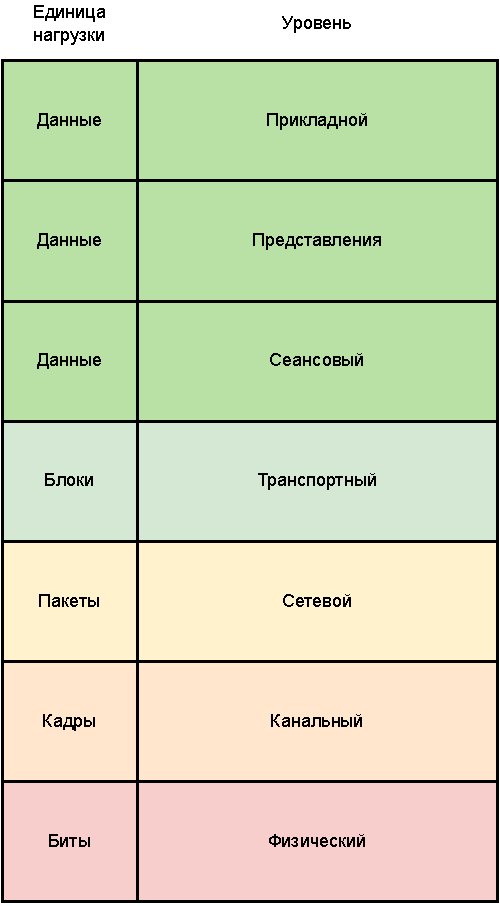
\includegraphics[scale=0.95]{img/osi.pdf}
	\caption{Модель OSI}
	\label{fig:osi}
\end{figure}

\begin{itemize}
	\item физический уровень: обеспечивает физическое соединение между устройствами и передачу битов по сети;
	\item канальный уровень: управляет надежной доставкой данных внутри локальной сети;
	\item сетевой уровень: обеспечивает маршрутизацию и передачу данных между различными сетями;
	\item транспортный уровень: отвечает за установление, управление и контроль надежной передачи данных между приложениями;
	\item сеансовый уровень: управляет установлением, поддержкой и завершением сеансов связи между устройствами;
	\item представительный уровень: обеспечивает преобразование данных в формат, понятный для приложений;
	\item прикладной уровень: предоставляет интерфейс для взаимодействия с приложениями.
\end{itemize}

Модель OSI широко используется при разработке и реализации сетевых протоколов, таких как TCP/IP, Ethernet и многих других. Она обеспечивает стандартизацию и согласованность в связи между различными системами и является основополагающей моделью для понимания работы сетевых сред.

\subsubsection{Транспортный уровень}

Транспортный уровень является третьим уровнем в сетевой архитектуре OSI. Он отвечает за передачу данных между конечными устройствами или хостами в сети. Основной задачей транспортного уровня является обеспечение эффективной и надежной передачи данных.

На транспортном уровне происходит сегментация данных на пакеты, каждый из которых содержит адрес отправителя и получателя, а также другую необходимую информацию. Пакеты передаются через различные узлы сети до достижения адресата.

\subsubsection{Протоколы транспортного уровня}

На транспортном уровне используются различные протоколы для обеспечения надежной передачи данных. Наиболее распространенными из них являются протоколы TCP (Transmission Control Protocol) \cite{TCP} и UDP (User Datagram Protocol) \cite{UDP}.

TCP является протоколом ориентированным на соединения. Он гарантирует доставку данных в правильном порядке и с контролем ошибок.

\begin{itemize}
	\item [---] TCP является соединительным протоколом. Он обеспечивает надежную, ориентированную на поток передачу данных между узлами в сети.
	\item [---] Для установления соединения TCP использует трехстороннее рукопожатие (three-way handshake), включающее отправку и получение пакетов SYN (synchronize) и ACK (acknowledge).
	\item [---] TCP контролирует порядок пакетов и гарантирует доставку данных без потерь, дублирования или повреждений.
	\item [---] Обеспечивает контроль нагрузки и управление потоком данных, чтобы избежать перегрузки сети.
	\item [---] TCP имеет встроенный механизм повторной передачи и контроля ошибок, что гарантирует целостность получаемых данных.
\end{itemize}

Протокол UDP используется в приложениях, где небольшие задержки более предпочтительны, например, в потоковой передаче видео и аудио. Основные особенности данного протокола:

\begin{itemize}
	\item [---] UDP является безсоединительным протоколом.
	\item [---] Не обеспечивает надежную доставку данных, контроль порядка пакетов или ретрансляцию потерянных пакетов.
	\item [---] UDP обеспечивает минимальное накладные расходы и более быструю передачу данных за счет отсутствия механизмов, используемых в TCP.
	\item [---] Он является хорошим выбором для приложений, где небольшие задержки важны, например, в реальном времени видео или голосовой связи.
	\item [---] Протокол UDP также удобен для широковещательной и многоадресной передачи данных.
	\item [---] В UDP-пакете нет гарантии доставки, но он прост и эффективен в простых сценариях, где периодическое обновление информации является приемлемым, а небольшие потери данных не критичны.
\end{itemize}

\subsubsection{Шифрование данных}

Шифрование данных является важным аспектом безопасности при передаче информации. Оно используется для защиты данных от несанкционированного доступа и предотвращения их изменения или подделки.

Шифрование данных может быть симметричным или асимметричным. В симметричном шифровании используется один и тот же ключ для шифрования и расшифрования данных.

Примерами симметричных алгоритмов шифрования является:

\begin{itemize}
	\item AES -- Advanced Encryption Standard \cite{AES};
	\item DES -- Data Encryption Standard \cite{DES}.
\end{itemize}

В асимметричном шифровании используется пара ключей: публичный и приватный. Публичный ключ используется для шифрования данных, а приватный ключ -- для их расшифровки. Это обеспечивает большую безопасность, так как приватный ключ хранится в секрете. Ниже представлены примеры наиболее популярных алгоритмов асимметричного шифрования:

\begin{itemize}
	\item RSA -- Rivest-Shamir-Adleman \cite{RSA};
	\item ECC -- Elliptic Curve Cryptography \cite{ECC};
	\item Diffie-Hellman \cite{diffie-hellman}. 
\end{itemize}

\subsection{Протоколы транспортного уровня с поддержкой шифрования}

\subsubsection{SSL / TLS}

\subsubsection{IPSec}

\subsubsection{DTLS}

\pagebreak
